\documentclass{standalone}

\usepackage{pgfplots,tikz,amsmath}
\begin{document}
		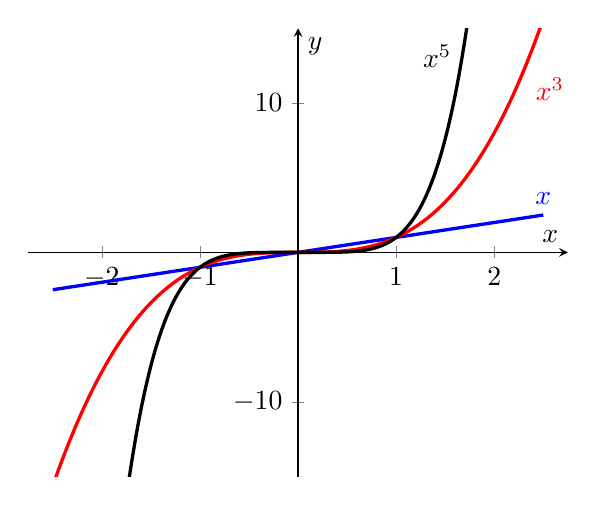
\begin{tikzpicture}%[scale=0.75]
			\begin{axis}[axis lines=center, xlabel={$x$}, ylabel={$y$},
				domain=-2.5:2.5,ymin=-15,ymax=15,xmin=-2.75,xmax=2.75]
				\addplot[smooth, very thick, blue, samples=150] {x}
					node[above]{$x$};
				\addplot[smooth, very thick, red, samples=150] {x^3}
					[below right] node[pos=0.9]{$x^3$};
				\addplot[smooth, very thick, black, samples=150] {x^5}
					[left] node[pos=0.57]{$x^5$};
			\end{axis}
		\end{tikzpicture}
		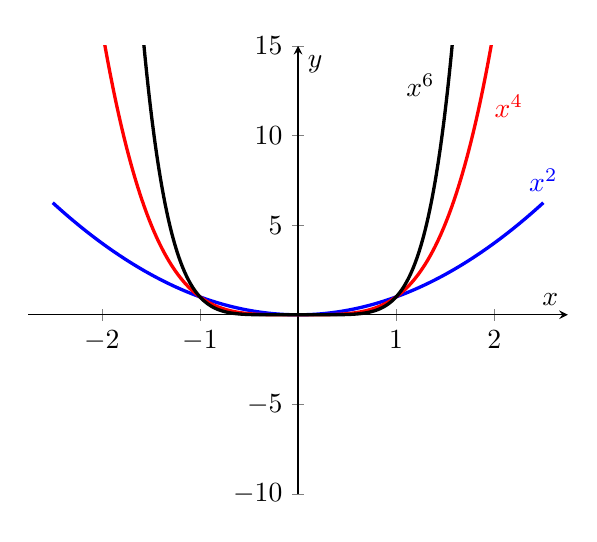
\begin{tikzpicture}%[scale=0.75]
			\begin{axis}[axis lines=center, xlabel={$x$}, ylabel={$y$},
				domain=-2.5:2.5,ymin=-10,ymax=15,xmin=-2.75,xmax=2.75]
				\addplot[smooth, very thick, blue, samples=150] {x^2}
					node[above]{$x^2$};
				\addplot[smooth, very thick, red, samples=150] {x^4} 
					[below right] node[pos=0.67]{$x^4$}; 				
				\addplot[smooth, very thick, black, samples=150] {x^6}
 					[above left] node[pos=0.525]{$x^6$};
			\end{axis}
		\end{tikzpicture}     
\end{document}
